\chapter{Performance}
\label{performance}

\section{Error Analysis of Params}

In order to do a thorough optimization, a total of 15 parameters would have to be varied simultaneously. 
Brief descriptions of these parameters can be found in \emph{parameters.txt} \coderef{parameters.txt}.
Such a large number of variables, however, leads to an intractable search space for optimization. 
To curb the computational burden we segmented parameter selection into a preliminary simulation step \coderef{simTaskScheduler.m} which identified sensitive and non-sensitive parameters and a fine tuning step which investigated these parameters further. 
During the analysis the following error metrics were used to compare trajectories.

\begin{equation*}LE = \underset{R,t,s}{\min} \sum_i (s R \cdot p_{est, i} + t - p_{GT, i})^2\end{equation*}
\begin{equation*}OE = \sum_i \text{rotMatToRotVec}(R^* \cdot R_{est,i} \cdot R_{GT, i}^T)^2\end{equation*}

Where $i$ is the index along the trajectory, $LE$ is the location error, $OE$ is the orientation error, $p_{GT}$ and $R_{GT}$ are the ground truth location and orientation, $p_{est}$ and $R_{est}$ are the estimated location and orientation and $R^*$ is the argument for R when $LE$ is minimal. 
The parameters $s$, $R$ and $t$ describe a generic similarity transformation. 
The function \emph{rotMatToRotVec} transforms the rotation matrix into a rotation vector of the form $\phi = \theta n$ \coderef{rotMatToRotVec.m}.

\section{Preliminary Simulations}

First, a sensible parameter configuration was guessed for each cluster. 
Then groups were fine tuned either manually or using simulation.  
Parameters which showed an increase in accuracy (deviation from ground truth, see chapter \ref{simulation}) and robustness (successful completion of run with varying other parameters) were selected at each step.

\medskip

Good Harris parameters (patch size = 9 and $\kappa$ =  0.08) where identified with low tracking loss. 
Moreover, the maximal number of candidates was determined to have low impact above 500. 
The sensitive parameters and ranges were narrowed down to 5 and are presented in table \ref{table:significant-param-tuning}.

\subsection{Parameter Fine Tuning}  

In this step the above parameters were varied in their ranges, while the other parameters were held constant and the OE and LE were recorded. 
1000 different combinations were tested in total and their results are shown in an error histogram in figure \ref{fig:error_histogram}. 
While the LE exhibits a large variance, the orientation error is much more concentrated in one peak. 
This shows that the location error is influenced much more by the variation of our parameters so from here on only the LE will be discussed.
In table \ref{table:significant-param-tuning} the three parameter combinations that lead to the lowest LE can be seen. \par
To compare the robustness of these candidates it is necessary to see how well the algorithm performs for similar parameter combinations. 
For this purpose histograms showing the distribution of the 10 best and 200 best results for each parameter were constructed and are shown in figure \ref{fig:best10} and \ref{fig:best200}.
It can be seen that \emph{triangulate\_max\_repr\_error} is very robust as 50\% (5 out of 10) of the top 10 share this value. 
It therefore makes sense that all top 3 candidates share this value. 
Also with \emph{nonmaximum\_suppression\_radius} all top 3 share parameters with the majorities from the top 10. 
This trend is supported further by the top 200 histograms.
The parameter \emph{tracker\_max\_bidirectional\_error} is shared by the top 3 and top 10. 
If we compare \emph{critical\_kp} we see that although two of the top three share the same value as the majority in the top 10 the best value is reached with a value of 100.
This can be explained by the fact that in the KITTI data set the second curve contains a dark patch which makes it hard to track key points. 
If there is no safety net many runs will just fail because they have too few landmarks to perform localization. 
A histogram displaying all failed runs illustrates this point in figure  \ref{fig:exceptions}. 
It shows that a parameter value of 0 leads to the majority of the exceptions which leads us to believe that this value is not robust although it may be optimal. 
The final parameter is \emph{add\_candidate\_each\_frame} which is robust to failure for all top 3 although not optimal for the best candidate.

\medskip

Due to its optimality and robustness against failure the best combination (see table \ref{table:significant-param-tuning}) was chosen.

\begin{table}[htp]
	\centering
	\caption{Parameter Fine Tuning: best three parameter combinations and their respective location error (LE). $LE_{max}$ : 23187, $LE_{min}$: 6664.9}
	\label{table:significant-param-tuning}
	\begin{tabular}{lrrrr}
		\hline
		\textbf{Parameters}                &         \textbf{Range} & \textbf{Best} & \textbf{2nd Best} & \textbf{3rd Best} \\ \hline
		$LE$                &                        &          6664 &              6987 &              7207 \\ \hline\hline
		nonmaximum\_supression\_radius     &                10:2:16 &            12 &                10 &                10 \\ \hline
		add\_candidate\_each\_frame        &              50:50:200 &           150 &               200 &               200 \\ \hline
		triangulate\_max\_repr\_error      & [0.5, 1, 2, 5, 10, 20] &             5 &                 5 &                 5 \\ \hline
		critical\_kp                       &       [0, 20, 50, 100] &           100 &                 0 &                 0 \\ \hline
		tracker\_max\_bidirectional\_error &      [2.1, 5, 9999999] &             5 &               2,1 &                 5 \\ \hline
	\end{tabular}
\end{table}

\begin{figure}[htp]
	\centering
	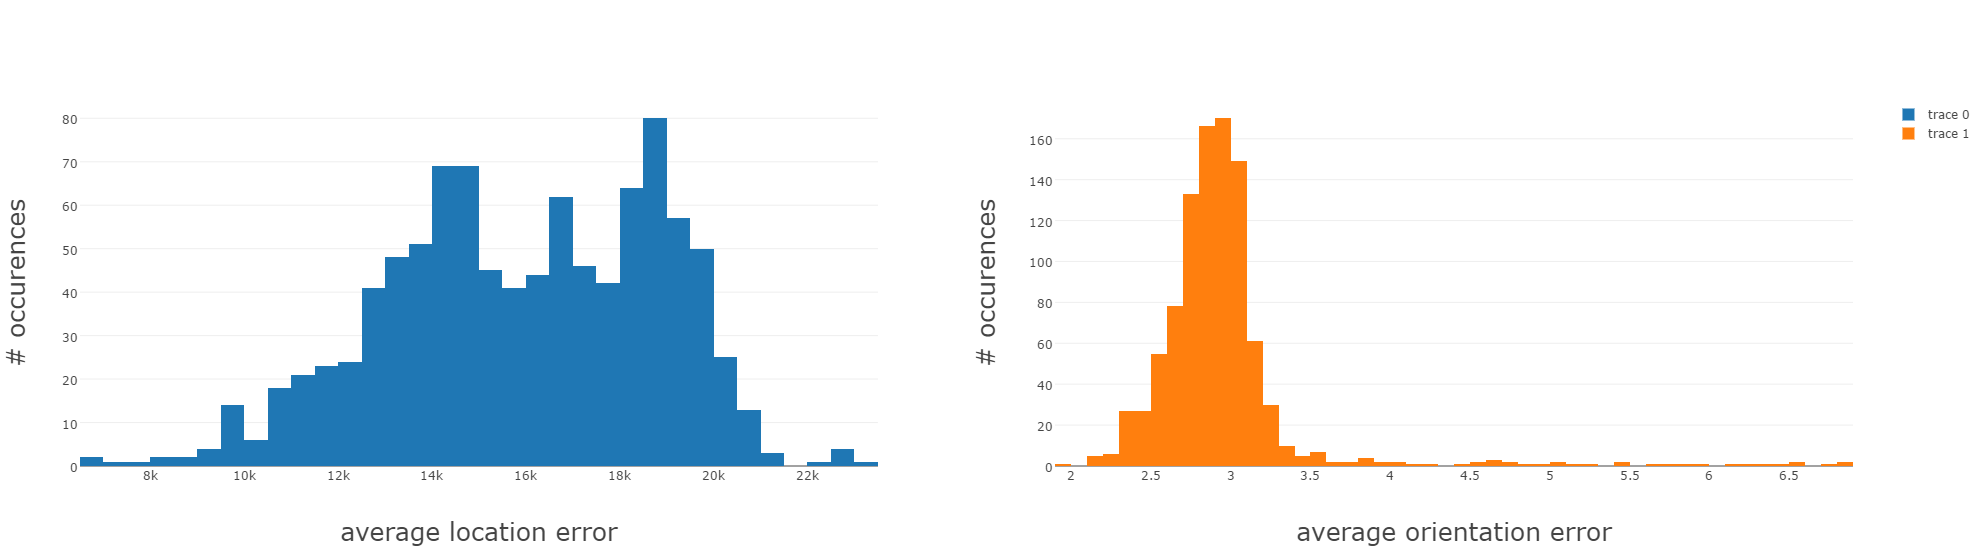
\includegraphics[width=1\textwidth]{figures/error_histogram}
	\caption{Distribution of the location error $LE$ and orientation error $OE$. 
	An outlier (23.79) was removed from the orientation errors. 
		$OE_{min}: 1.97$, 
		$OE_{max}: 23.79$,
		$OE_{med}: 2.89$,
		$LE_{min}: 6664.9$,
		$LE_{max}: 23187.5$,
		$LE_{med}: 16059.0$}
	\label{fig:error_histogram}
\end{figure}

\begin{figure}[htp]
	\centering
	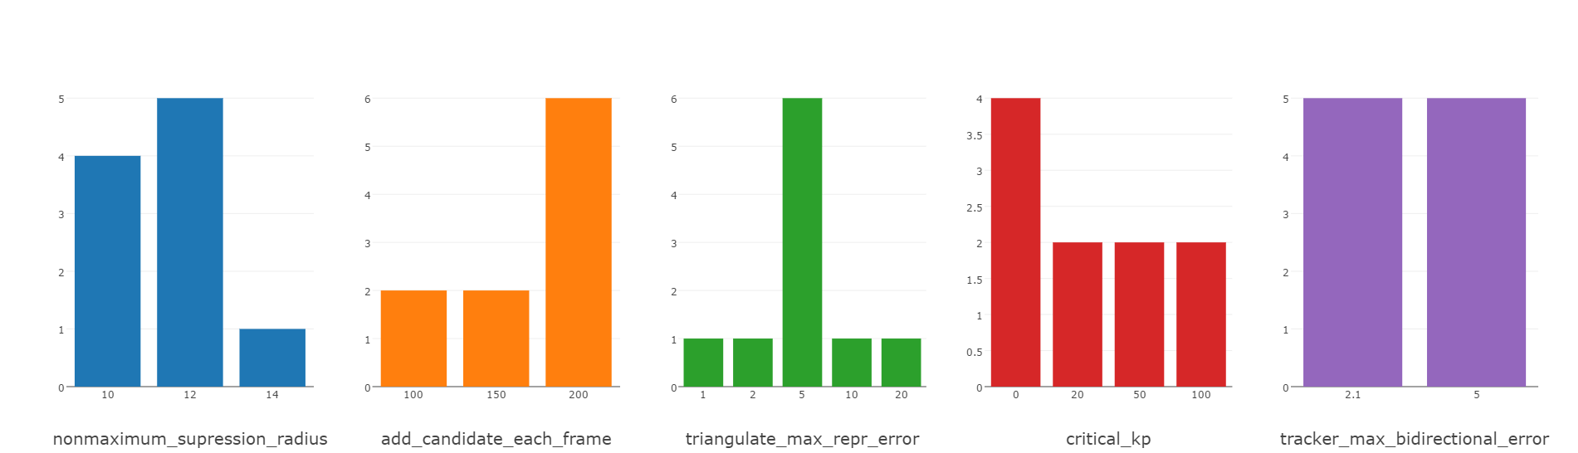
\includegraphics[width=1\textwidth]{figures/best10}
	\caption{Parameter distribution of the best 10 results  (15\% of the dynamic range).}
	\label{fig:best10}
\end{figure}

\begin{figure}[htp]
	\centering
	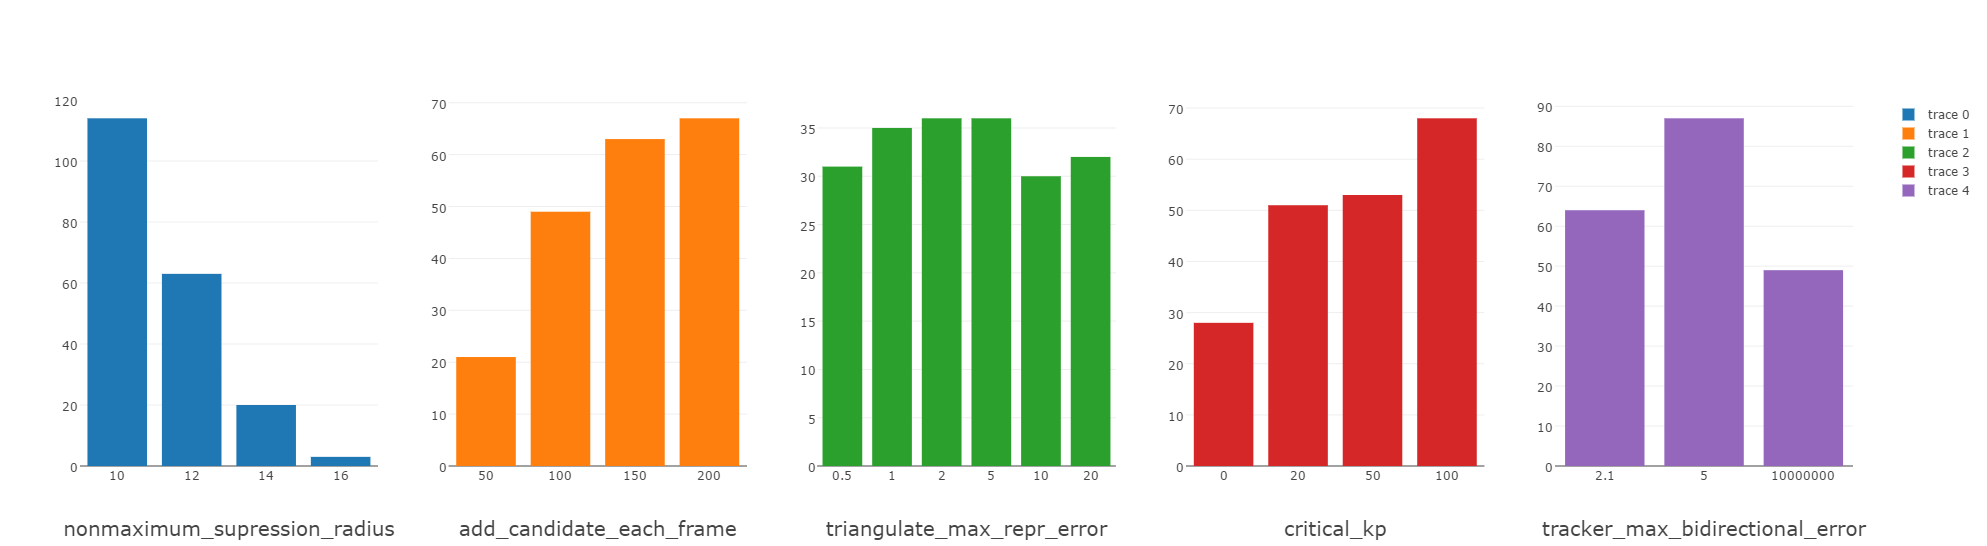
\includegraphics[width=1\textwidth]{figures/best200}
	\caption{Parameter distribution of the best 200 results  (40\% of the dynamic range).}
	\label{fig:best200}
\end{figure}

\begin{figure}[htp]
	\centering
	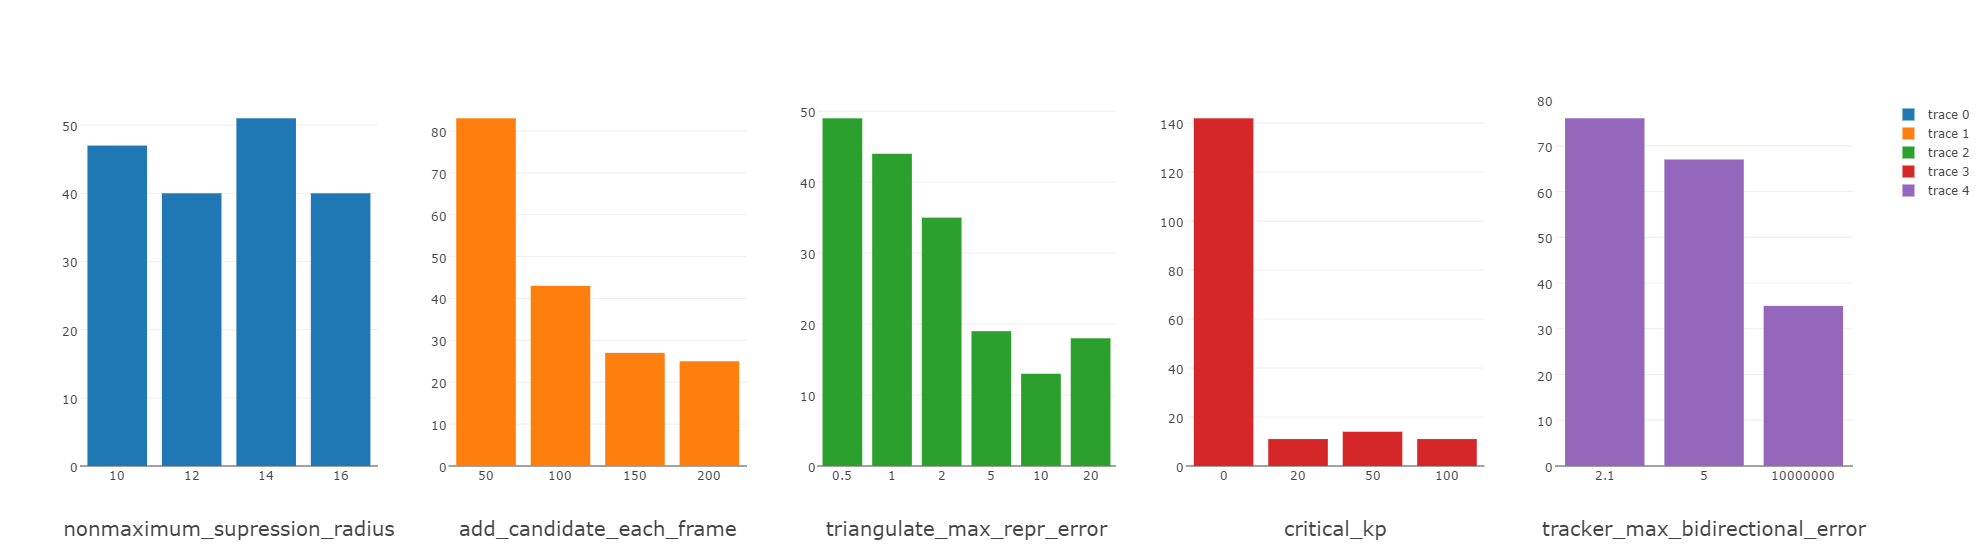
\includegraphics[width=1\textwidth]{figures/exceptions}
	\caption{Parameter distribution of all runs that terminated due to excessive loss of key points. }
	\label{fig:exceptions}
\end{figure}